\pdfoutput=1
% Synthetic acceptance fixture (MIT, part of rstex2word). It mirrors the
% constructs of AI-assisted arXiv papers such as arXiv:2610.32813: TikZ
% figures kept in \input files, stacked pictures in one figure*, captions
% built with \protect\input, nested \input paths relative to the main file,
% headings with several \label keys, url-package \path, and the end-matter
% commands of a two-column layout.
\documentclass[10pt,twocolumn,letterpaper]{article}
\usepackage[margin=0.75in]{geometry}
\usepackage{times}
\usepackage[dvipsnames]{xcolor}
\usepackage[numbers,sort&compress]{natbib}
\usepackage[hyphens]{url}
\usepackage{booktabs,amsmath,amssymb,graphicx}
\usepackage{tikz}
\usepackage{balance}
\usetikzlibrary{positioning,arrows.meta,fit,calc,plotmarks}
\usepackage[colorlinks,allcolors=blue]{hyperref}
\newcommand{\ours}{\textup{Fixture}}
\title{Rendering TikZ in Word: an acceptance fixture}
\author{A. Author}
\date{}

\begin{document}
\maketitle

\begin{abstract}
\ours{} checks that every TikZ picture of a figure reaches the document.
\end{abstract}

\section{Introduction}
\label{sec:intro}
Figure~\ref{fig:pipeline} shows the pipeline; Table~\ref{tab:results}
lists the results and Appendix~\ref{sec:alias} the protocol. Raw data are
in \path{generated/results_raw.json}. We follow prior work~\citep{knuth1984}.

\begin{figure*}[t]
\centering
\definecolor{stage}{RGB}{37,99,235}
\begin{tikzpicture}[node distance=8mm,font=\small,
  box/.style={draw=stage,rounded corners=1mm,minimum width=22mm,minimum height=7mm}]
\node[box] (src) {LaTeX source};
\node[box,right=of src] (ir) {IR};
\node[box,right=of ir] (docx) {Word document};
\draw[-{Stealth}] (src) -- (ir);
\draw[-{Stealth}] (ir) -- (docx);
\node[draw=black!30,dashed,fit=(src)(ir)(docx),inner sep=2mm] {};
\end{tikzpicture}

\caption{Pipeline overview. \protectEach stage is one crate; the caption text comes from a generated file.
}
\label{fig:pipeline}
\end{figure*}

\section{Results}
Table~\ref{tab:results} is generated; its path is resolved against the main
document's directory, as TeX does.
\begin{table}[t]
\centering
\caption{Results on the fixture benchmark.}
\label{tab:results}
\begin{tabular}{lrr}
\toprule
Variant & Success (\%) & Tokens (k) \\
\midrule
Full & 93.77 & 13.17 \\
W/o reuse & 81.20 & 18.03 \\
\bottomrule
\end{tabular}
\end{table}



\begin{figure*}[t]
\centering
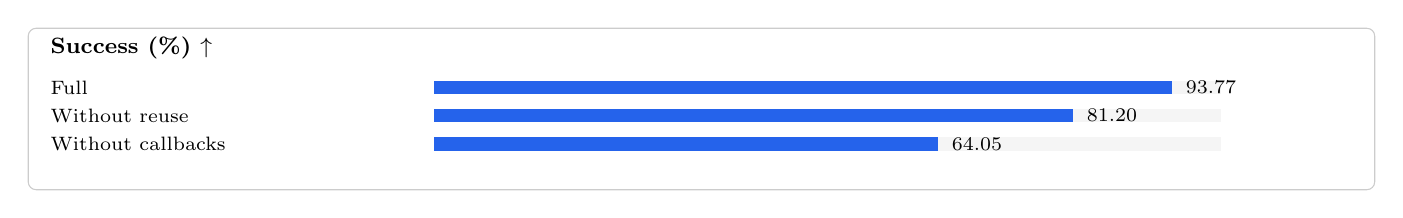
\begin{tikzpicture}[x=1cm,y=1cm,font=\scriptsize]
\definecolor{bar}{RGB}{37,99,235}
\draw[black!20,rounded corners=1mm] (0,0.75) rectangle (17.1,-1.30);
\node[anchor=west,font=\bfseries\footnotesize] at (.16,.50) {Success (\%) $\uparrow$};
\foreach \label/\value/\y in {Full/93.77/0, Without reuse/81.20/-0.36, Without callbacks/64.05/-0.72} {
  \node[anchor=west] at (.16,\y) {\label};
  \fill[black!4] (5.15,\y-0.085) rectangle (15.15,\y+0.085);
  \fill[bar] (5.15,\y-0.085) rectangle ({5.15+\value/10},\y+0.085);
  \node[anchor=west] at ({5.20+\value/10},\y) {\value};
}
\end{tikzpicture}

\par\vspace{2mm}
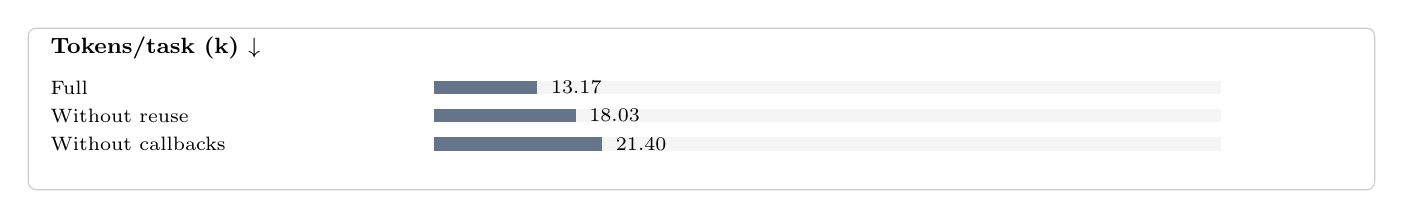
\begin{tikzpicture}[x=1cm,y=1cm,font=\scriptsize]
\definecolor{bar}{RGB}{100,116,139}
\draw[black!20,rounded corners=1mm] (0,0.75) rectangle (17.1,-1.30);
\node[anchor=west,font=\bfseries\footnotesize] at (.16,.50) {Tokens/task (k) $\downarrow$};
\foreach \label/\value/\y in {Full/13.17/0, Without reuse/18.03/-0.36, Without callbacks/21.40/-0.72} {
  \node[anchor=west] at (.16,\y) {\label};
  \fill[black!4] (5.15,\y-0.085) rectangle (15.15,\y+0.085);
  \fill[bar] (5.15,\y-0.085) rectangle ({5.15+\value/10},\y+0.085);
  \node[anchor=west] at ({5.20+\value/10},\y) {\value};
}
\end{tikzpicture}

\caption{\protectQuality and cost of the three variants. Top: success rate; bottom: tokens per task.
}
\label{fig:bars}
\end{figure*}

Figure~\ref{fig:bars} stacks two pictures; the cost model is $c = n\,t$
\citep{lamport1994}.

\clearpage
\nobalance
\typeout{MAIN_BODY_NEXT_PAGE=\thepage}
{\small
\bibliographystyle{plainnat}
\bibliography{refs}
}

\clearpage
\onecolumn
\appendix
\section{Protocol}
\label{sec:protocol}
\label{sec:alias}
The protocol section carries two labels; both resolve to it.

\end{document}
